The main conference begins!

\subsection{Tom Griffiths on Rational Use of Cognitive
Resources}

Joint work with Falk Lieder, Fred Callaway, and Michael Chang. \\

This crowd: AI/Neuro/pscychology, leads to diverse perspectives on intelligence and cognition.


\subsubsection{A Paradox: Human Cognition is Inspiring (AI) and Embarrassing (Psychology)}

{\bf Recent trend:} exponential increase in compute required for major breakthroughs (from AlexNet to ALphaGo Zero, plot OpenAI blog post). \\

$\ra$ Recall deep blue vs. Kasparov. Fundamental computing difference: Kasparov evaluating 1 move per second vs. Deep Blue, evaluating 100,000 positions per second. \\

**People can do more with less. \\


Conclusion from the AI perspective: people are amazing! We can solve all sorts of cognitive challenges, all with the same system. \\

Conclusion from the psychology perspective: humans are embarrassing! See books: ``predictably irrational", ``inevitable illusions", ``how we know what isn't so", and ``the haphazzard construction of the human mind". \\

{\bf Paradox:} How can we be inspiring enough that AI reseachers are excited about us, while silly enough that psychologists are embarrassed by us.

\subsubsection{Toward Resolving the Paradox: Resource Rationality}

Toward resolving the paradox:
\begin{enumerate}
    \item Humans have limited cognitive resources~\cite{simon1972theories}.
    \item We do a good job of using those resources~\cite{lieder2019resource}.
\end{enumerate}

\ddef{Rational Decision Theory}{Take the action with highest expected utility:
\[
\argmax_a \bE[U(a)].
\]}


But, ignores computational cost. So:
\newpage
\ddef{Bounded Optimality~\cite{russell1994provably}}{Use the strategy that best trades off utility and computational cost:
\[
\argmax_\pi \left[\max_a \bE[U(a) \mid B_T] - \nsum \tx{cost}(B_t, C_t)\right].
\]}

So, decision theory: ``do the right thing", and bounded optimality: ``do the right thinking". \\

We can then pose the following: when we take into account the cost of computation, what kinds of heuristics/biases are resource rational? \\

Two examples: 1) Anchoring and adjustments~\cite{lieder2012burn}, or 2) Availability of extreme events~\cite{lieder2018overrepresentation}. \\

Q: How do we derive optimal strategies? \\

Key insight: the problem of choosing a cognitive strategy to follow can be described as a sequential decision problem with computations as actions. In:
\[
\argmax_\pi \left[\max_a \bE[U(a) \mid B_T] - \nsum \tx{cost}(B_t, C_t)\right],
\]
we let $\pi$ denote a choice of computations to use to solve a problem. \\

$\ra$ This can be formulated as a ``meta-level" MDP, and solved using methods from RL (and other methods more tailored to these meta-level problems). \\

\ddef{Meta-Level MDP~\cite{hay2014selecting}}{A sequential decision problem where states are beliefs of the agent and actions are the choice of computations to execute.}

A policy describes the sequence of computations an agent will use to solve a particular problem. \\

{\bf Example 1:} Mouselab paradigm~\cite{payne1993adaptive}. A game where people click different cells/gambles that yield different outcomes with different probabilities.

\begin{itemize}
    \item Finding: people use the ``take the best" strategy (outcome with highest probability). How do people choose a strategy?
    \item Translate this problem into a meta-level MDP! State space corresponds to beliefs people have about payoffs for each clickable cell in the game. Each click is associated with some cost, costs accumulate. Can then derive the optimal cognitive strategy under different circumstances.
    \item Finding: the ``take-the-best" strategy is optimal under some conditions! (stakes are very low). But, for compensatory low-stakes problems, take-the-best is no longer optimal.
\end{itemize}

{\bf Example 2:} Same ideas extend to {\it planning}. Now an agent has to navigate through a weighted graph to find the lowest cost path.
\begin{itemize}
    \item People have to learn the edge weights of the graph (that is, they have to explore).
    \item Idea: Can again translate this problem into a meta-level MDP.
    \item Finding: people are {\it adaptively} deciding when and how much to explore. Displayed by people {\it and} the optimals strategy (to the meta-level MDP), but not found in most search algorithms (like BFS/DFS).
\end{itemize}

\subsubsection{Resource Rationality in AI and Psychology}

Resource Rationality and Psychology:
\begin{itemize}
    \item **Cognitive Psychology is about {\it processes}, which we can now derive from {\it problems} (by translating it into this meta-level MDP).
    \item Forges a question to RL that sets up compelling questions and answers:
    \begin{itemize}
        \item Strategy learning as RL (model-based and model-free)
        \item Shaping as a means of improving cognition
        \item Neuroscience hypotheses about cognition vs. action
    \end{itemize}
\end{itemize}

Resource Rationality and AI:
\begin{itemize}
    \item Considering how to allocate ognituve resources means considering how to reuse resources
    \item Critical part of creating learners that are able to perform heterogeneous tasks.
    \item Problems that don't look like metareasoning can be expressed as metalevel MDPs.
    
    Example: learning the structure of deep neural nets~\cite{peterson2018evaluating}
\end{itemize}

Often, learning structures leads to {\it compositional generalization}~\cite{chang2018automatically}.\\ 

Example: Translate from English to Spanish. But, already know how to translate English to French and French to Spanish, can use this to translate English to Spanish (via French). \citet{chang2018automatically} study translating from pig latin into spanish by picking up on relevant compositional structure. \\


\dbox{{\bf Conclusions:}
\begin{enumerate}
    \item Finding computationally efficient strategies is a key component of human intelligence.
    \item Capturing this capacity in machines can lead to systems that are capable of flexible generalization and more efficient learning.
    \item Formulating rational models of the use of cognitive resources sets up a new direction for RL and decision making.
\end{enumerate}}

\spacerule

\subsection{Will Dabney on  A Distributional Code for Value in
Dopamine-Based RL}

Joint with Zeb Kurth-Nelson, Nao Uchida, Clara Starkweather, Demis Hassabis, Remi Munos, and Matthew Botvinick. \\

To start: think back to our shared (across neuro/AI) roots in TD learning.
\[
V(s) \la V(s) + \alpha(r + \gamma V(s') - V(s)).
\]
This model is the baseline {\it across both fields}. \\

Proposal of the model: global value estimate $\hat{V}$. In Neuroscience: neurons are reporting a prediction error against this global estimate. Neurons move toward estimating the mean value of the future returns. \\
    
    $\ra$ Key: Dopamine neurons scale their values in positive and negative directions. This allows them to estimate the mean. \\


{\bf This Work:} New idea, ``distributional" TD-Learning. Dopamine neurons actually scale their predictions in {\it different ways} across the population. \\

$\ra$ Different neurons are learning different statistics about the prediction of these errors/values. \\

Point from AI: distributional RL tends to help in complex environments!~\cite{bellemare2017distributional}. \\

\dbox{{\bf Central Q:} Can this distributional perspective help our understanding of dopamine prediction error in the brain?}


\begin{figure}[h!]
    \centering
    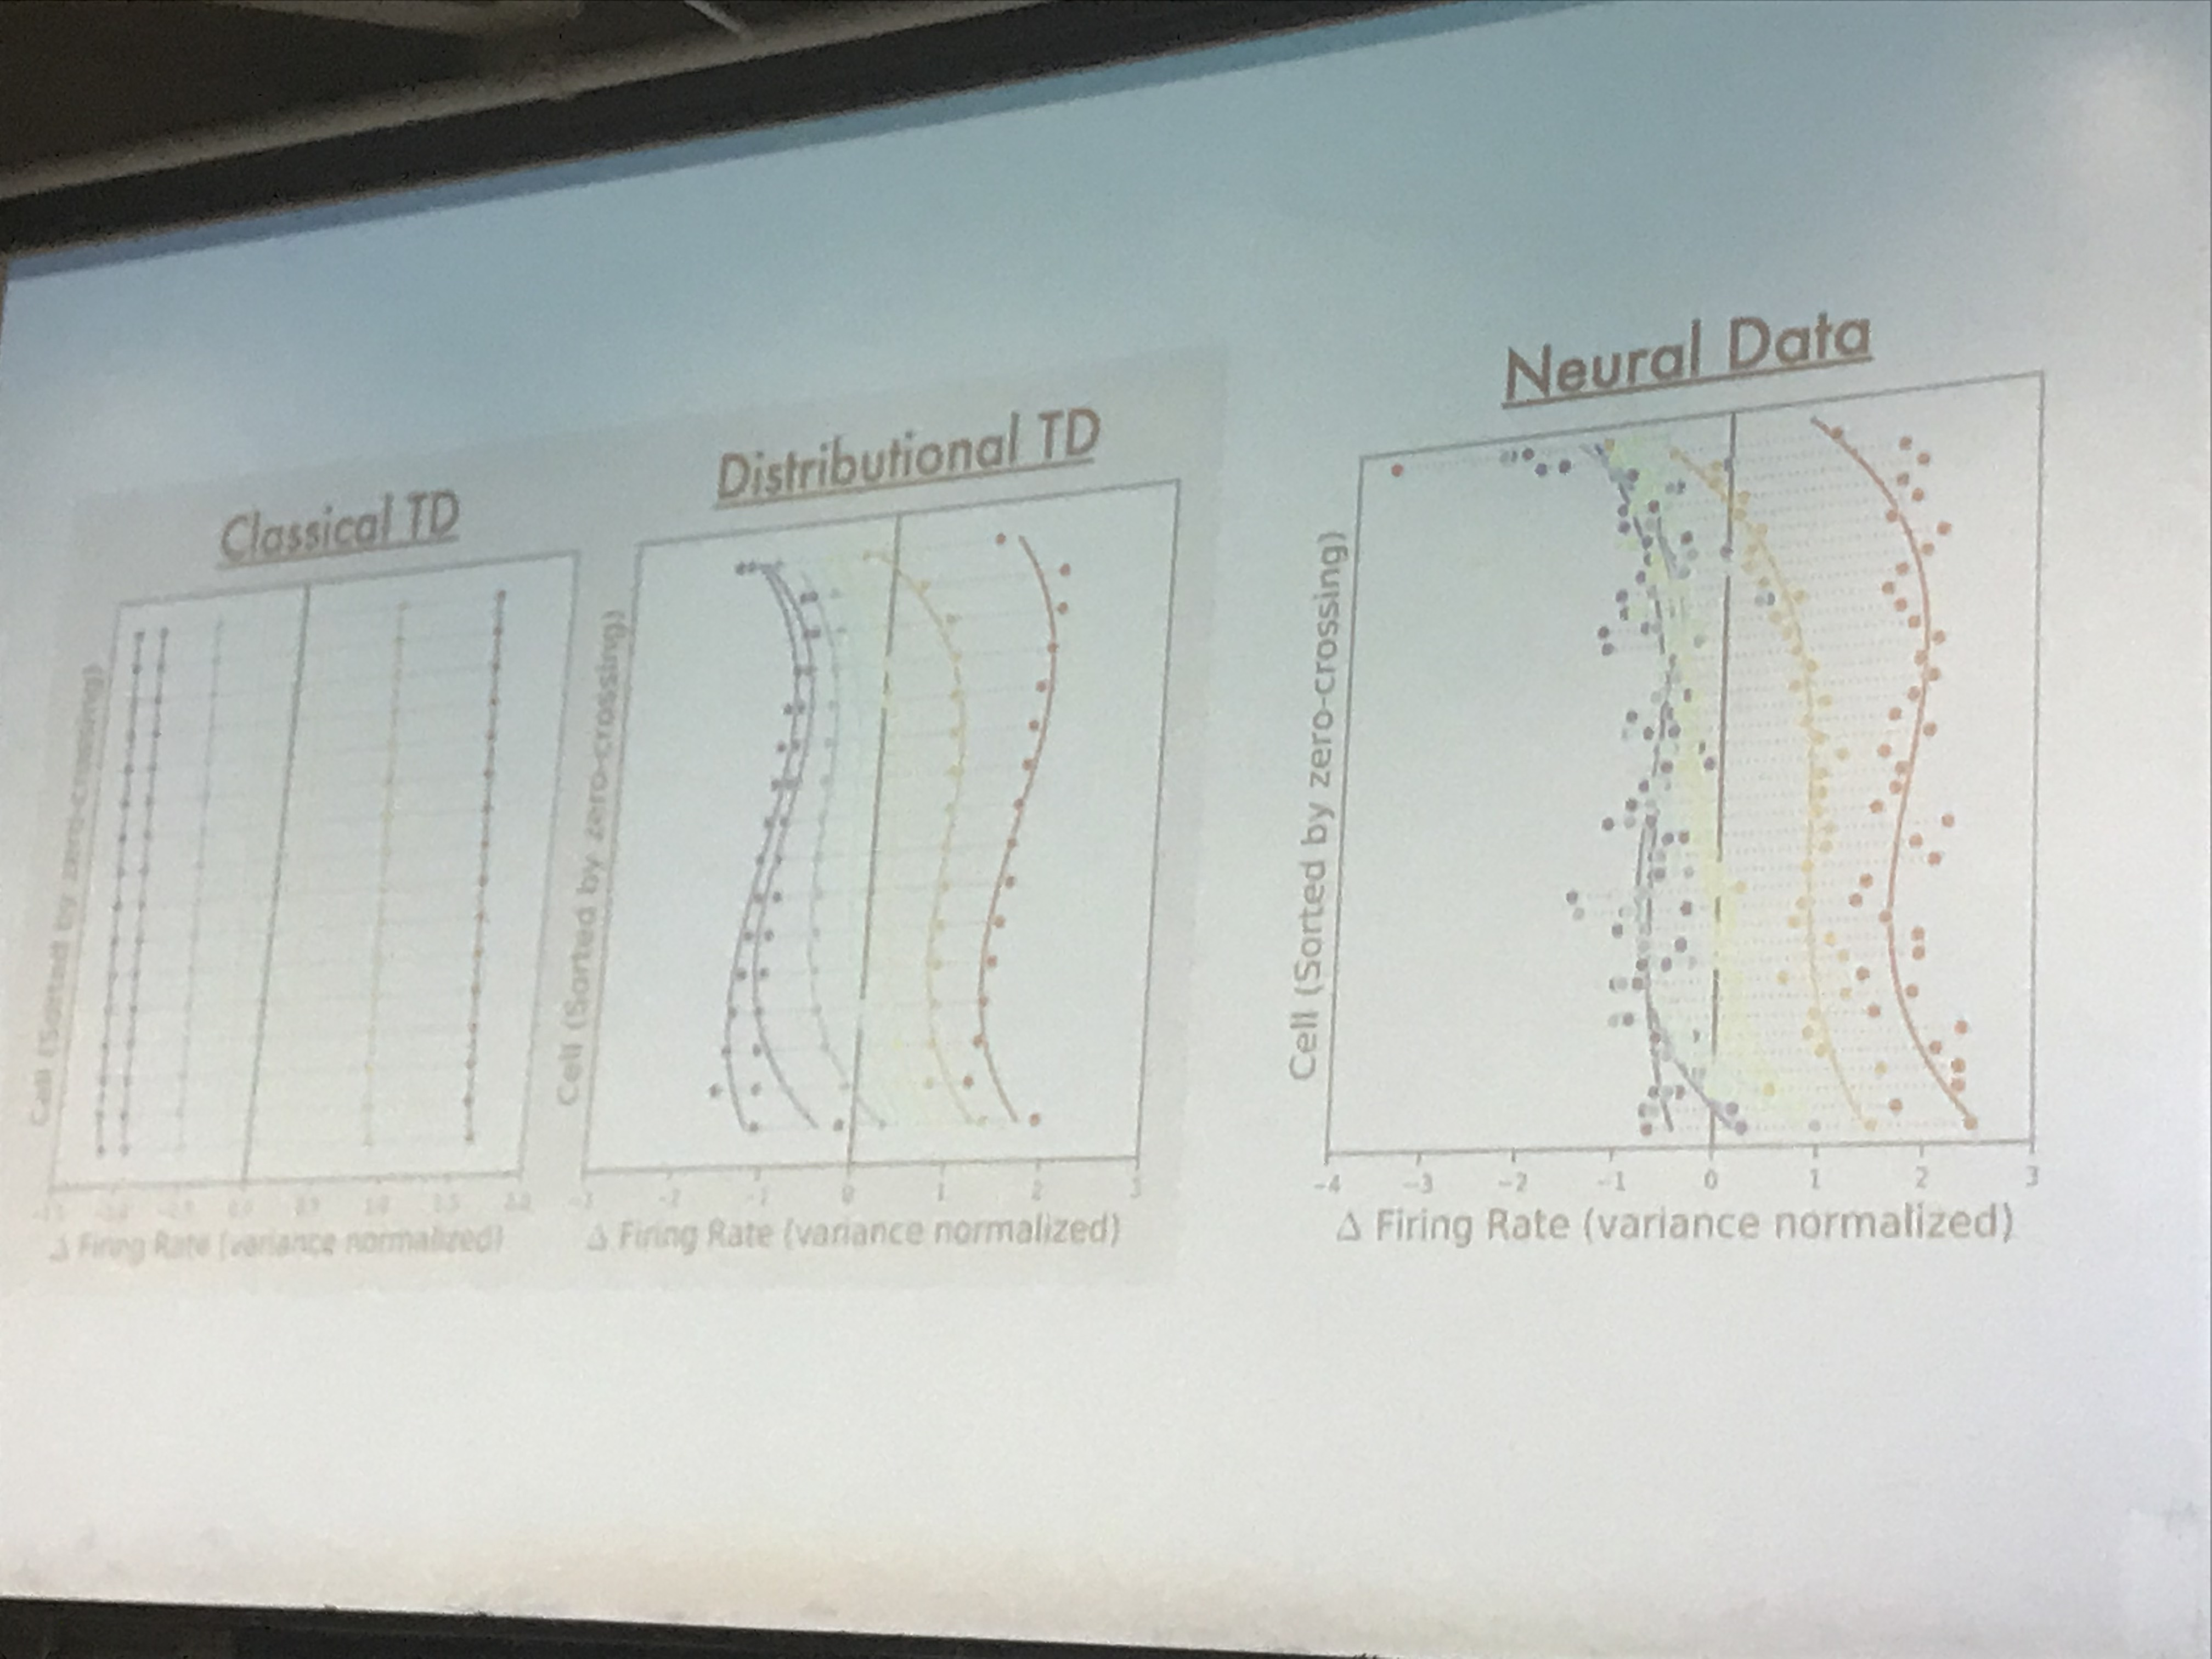
\includegraphics[width=0.5\textwidth]{images/dist.JPG}
    \caption{Predictions by classical TD view of dopamine neurons (left), distributional view (middle), and results (right).}
    \label{fig:dist_td}
\end{figure}

{\bf Experiment 1:} 
\begin{itemize}
    \item An animal is given a stimuli (odor) then given juice of different degrees from $[1:7]$ (more is better). In the second tasks, there is some probability of getting reward/juice.
    \item Classical Finding: when the reward given is below their average, then the TD error is positive (predicts error). When it's above, TD error (found in neurons) is negative.
    
    \item {\bf Main comparison:} distributional take (different neurons predict different statistics of the distribution of reward) vs. classic TD (all dopamine neurons should have the same firing rate).
    
    \item New Finding: the actual firing rates are very well predicted by the distributional perspective, not the classical view. See Figure~\ref{fig:dist_td}
\end{itemize}


{\bf Experiment 2:} Further exploration over whether dopamine neurons {\it agree} in their predictions (and so are all responsible for monitoring the same signal), or if they disagree (and are thus picking up on different statistics of the distribution). \\


$\ra$ Further find diversity in asymmetry of predictions as scaling in DPEs is applied.

\spacerule


\subsection{Marlos Machado on Count Based Exploration with the Successor Representation}
\label{sec:mr}

Joint with Marc G. Bellemare and Michael Bowling. \\

{\bf Focus:} exploration problem in computational RL. That is, learn about the world by only seeing the consequences of each chosen action. \\

$\ra$ Typical trend: use random exploration, such as:
\[
\pi_{\hat{Q},\eps} (s) = \begin{cases}
\argmax_a \hat{Q}(s,a)& 1-\eps \\
\tx{Unif}(\mc{A})& \eps \\
\end{cases}
\]
But: acting randomly leads to very inefficient exploration. In a simple grid world, can take around 800-900 steps on average. \\

Main result: the norm of the {\it successor representation} while it is being learned, implicity encodes state visition counts. Thus, it can be used as an exploration bonus.
\ddef{Successor Representation~\cite{dayan1993improving}}{A representation of state that captures proximity in space over time between states. %Something like: two states are similar in representation if they can reach each other easily (under some policy).
More formally;
\[
\psi_\pi(s,s') = \bE_\pi\left[\sum_{t=0}^\infty \gamma^t \indic\{s_t = s' \mid s_0 = s\}\right]
\]}

Also: nice generalizations to function approximation, nice connections to DP~\cite{wang2007dual}, eigenvectors of SR equivalent to slow feature analysis, and more. \\

Q: Where did these ideas come from? \\

A: Well, originally look at it from the perspective of learning the connectivity of the graph of the MDP. After only a few episodes (100 or so in grid worlds) already picks up on enough structure to use for exploration. \\

Can combine with Sarsa via an exploration bonus:
\[
Q(s,a) \la Q(s,a) + \alpha \left[\left(r + \frac{1}{||\psi(s)||_2}\right) + \gamma Q(s',a')\right].
\]

Model-free RL: the norm SR can be used as an exploration bonnus (yields more efficient exploration in river swim like problems). \\

Model-based RL: can also combine with efficient exploration algorithms like $E^3$, R-Max~\cite{brafman2002r}, and so on.\\

$\ra$ But can also combine with function approximation. 
\begin{itemize}
    \item Idea: use a deep network to yield some state features, $\phi$.
    \item Use $\phi$ to predict both $\hat{Q}$ {\it and} $\psi$.
\end{itemize}

Exploration in Atari Games:  DQN yields low scores on hard exploration games, while adding the SR to DQN gives a boost in most cases. \\

$\ra$ Claim is not this dominates other exploration methods, but rather that it's a simple general idea that can enhance exploration. \\

\spacerule


\subsection{Will Dabney on Directions in Distributional RL}

Let's start with a high level definition of distributional RL:
\ddef{Distributional RL~\cite{bellemare2017distributional}}{Do RL! But, with more statistics than the mean.}

That is: given that there is a return distribution out there in the world, we want to estimate some statistics about this distribution. Usual tool: Bellman Equation ($V = R + \gamma V'$). \\

But, what happens when we go beyond estimation of the mean? \\

Q: How many distributions are consistent with the mean I'm estimating? \\

A: Well, infinitely many! \\

Q: But what if we add more statistics? (Like other moments!) \\

A: Well, that will trim this space of distributions down to something more tractable/reasonable. \\

The distributional RL update, assuming the return distribution is a random variable:
\[
Z^\pi(x,a) := R(x,a) + \gamma Z^\pi(X_1, A_1).
\]
Many such statistics of interest!
\begin{itemize}
    \item {\it Mean:} Regular RL! Just estimating the mean.
    \[
    \bE[Z^\pi(x)]
    \]
    \item {\it Categorical Distr. RL:} A traditional ML approach to estimating the distribution via regression (but really turn it into classification).
    
    \[
    \Pr(Z^\pi(x) \leq z_k)
    \]
    
    $\ra$ Tells us: will the return in my distribution be more than some value?
    
    \item {\it Quantile Regression Distr. RL:} Think about minimizer for absolute loss $\ra$ median! If we tilt the loss, we force the solution to be something other than the median.
    \[
    F_{Z^\pi(x)}^{-1}(\tau_k)
    \]
    \item Others: unimodal gaussian/laplace, others.
\end{itemize}

\subsubsection{Why Does Distributional RL Help?}

Q: Why is distributional RL helping? \\

A1: Well, per the work by~\citet{lyle2019comparative}, the updates between classical/distributional RL are effectively identical in many settings. \\

A2: It could also lead to take the wrong answer if distribution is skewed~\cite{rowland2019statistics}. \\

$\ra$ So, it doesn't seem like it {\it should} help. But, lots of evidence that it does! See, for instance, Rainbow~\cite{hessel2018rainbow}.\\

Key Challenges:
\begin{enumerate}
    \item {\it Optimization Stability:} Hard to keep the optimization process stable.
    \item {\it Representation Learning:} Learning the right representation is hard!
\end{enumerate}

$\ra$ These both seem like cases where distributional RL can help! \\


\citet{imani2018improving} showed that using distribution loss for regression doesn't always help in supervised learning! But, in RL, there are special properties that might lead to better representation learning. \\

\citet{van2016learning} introduce the Pop-Art algorithm. Study how optimization becomes very instable when data is presented over many orders of magnitude. Pop-Art able to overcome this issue and yield more stable updates.\\

$\ra$ Idea is that being aware of the magnitude of the error can yield more stable updates. \\

So, toward stabilizing optimization: 1) Distribution loss can be less sensitive to magnitude of errors, and 2) RL, a non-stationary regression problem, can look a lot like stochasticity to sample based algorithms. \\

**Way to think about this; the value function is a stepping stone that acts as a means of moving on to the next, better policy. \\

$\ra$ Often we {\it overfit to the current stepping stone}, instead of moving on from it at the right time. \\

Should ask: how well can my value function fit future value functions, not just the current ones?


{\bf Hypothesis:} Distributional RL is doing something to shape the representation to be robust with respect to future value functions! It does this by providing support to shape future and past value functions.\\

Experiments to explore this claim: how well do different learned representations generalize to {\it future} value functions? \\

$\ra$ Finding: Really strong correlation between how well you can fit future value functions and how well you perform on a set of tasks.

\subsubsection{What Can We Do With Distr. RL?}

Now, let's returning to original Q: What can we do with it? \\

Some directions:
\begin{itemize}
    \item Risk-Sensitive behavior: Using estimate of distribution of return can be important for adapting risk profile.
    \item From economic paradoxes (allias, st petersburg, ellsberg)---can we understand the statistics that would imply these sorts of decision making?
    \item Hyperbolic discounting: if discount is a probabiliy, not a scaling.
\end{itemize}


{\bf The Virtuous Circle of RL:} great benefit of having a huge overlap between AI/neuroscience/psychology (and others). An old story: blind people studying an elephant~\cite{saxe1994blind}. \\

$\ra$ But, we have a much better shot at understanding the nature of the entity we're studying. \\

Directions in Distributional RL:
\begin{itemize}
    \item For AI: technique for improving stability/learning, improv understanding of representation learning in RL
    \item For Neuroscience: can distributional RL help explain variability in dopamine activity? do model-free and model-based distribution estimates get combined
    \item For Psychology: broad class of risk-sensitive policies, but challenging to analyze. Errors in risk-sensitive behavior tell us about underlying mechanisms.
\end{itemize}

\spacerule


\subsection{Anna Konova on Clinical Decision Neuroscience}

{\bf Goal:} Highlight the ways in which work in decision neuroscience can be relevant to other areas! \\

$\ra$ Focus: Understanding drug addiction. \\

\ddef{dsm-5 criterion}{11 steps of a substance abuse disorder (1 use for longer than indended, 2 more than one attempt to cut down, and so on).}

Experiment: try to capture risk propensity by having subjects play tasks.
\begin{itemize}
    \item Subjects presented two bags. The first has guaranteed \$5 in it, the other has a 50/50 chance of giving 0 vs. \$10.
    \item Modeling risk preferences: money is valued differently for different people. So, for each person, a function that maps ``objective value" to subjective value (relative increase in satisfaction with each increase in \$).
    
    $\ra$ This function is the utility function $U(v) = v^{\alpha}$.
    
    \item Expected utility theory with risk, then:
    \[
    \bE[U(v)] = pv^{\alpha}
    \]
    
    But how about risk? Well, $\alpha$ can capture that.
    
    \item Hypothesis: drug users are more risk tolerant than non drug users.

    $\ra$ Findings: cocaine users have higher risk tolerance, schizophrenia patients have normal risk tolerance, and those with anxiety disorders have lower risk tolerance.
\end{itemize}

Addiction is characterized by a cycling pattern:

Q: What are the cognitive mechanisms that underlie this cycling process? \\

A: To address this question, we need to better understand these cognitive mechanisms. \\

$\ra$ Focus on opiod epidemic, and specifically on opiod users that have recently entered rehab-like programs. \\

Experiment:
\begin{itemize}
    \item Setup: again consider a set of bags of different risk profiles.
    \item Modify the model with a new parameer $\beta$, that indicates a subject's ambiguity tolerance:
    \[
    \bE[U] = \left(p-\beta \frac{A}{2}\right)v^{\alpha}.
    \]
    
    \item Studied risk and ambiguity tolerance over seven months of prior opiod users, and tested whether they returned to drug use (along with MRI scans and some other data).
    
    \item Data enables connection between these tolerances and actual behavior.
    
    \item Findings:
    \begin{itemize}
        \item As a group, opiod users were more risk tolerant than controls.
        \item What about fluctuating drug use vulnerability? (cycle from before). Turns out that there is no relationship to changes in risk/ambiguity tolerance.
        
        \item Ambiguity tolerance independently predicts use beyond changes in clinical status.
        
        $\ra$ Moreover: the size of the effect is similar to the effect of a craving (that is, it's clinically meaningful).
        
        \item Can plot/study the effect of ambiguity tolerance to use heroine.
        \item Lots of fluctuation in ambiguity tolerance over time.
    \end{itemize}
\end{itemize}

Interpretation of the above data: more tolerance of ambiguity outcomes might lead to more tolerance of potential outcomes of drug use. \\

$\ra$ This interpretation requires that the effects discovered generalize well. Thus, a follow up study: this time unstructured study of opiod users from a variety of backgrounds. \\

{\bf Finding:} Similar pattern emerges. Increase in ambiguity tolerance continue to be positively predictive of continued future use, even when accounting for lots of other variables. \\

Q: How does the brain reflect increased ambiguity tolerance? \\

A: Collected fMRI data from many subjects during the trials. From their choice history, can obtain $\alpha, \beta$ over time for each subject. Moreoever, from the fMRI, can associate neural data with $\alpha, \beta$. \\

$\ra$ Finding: observe subjective value signals where we expect to see them in all subjects. Thus, clearly value coding in particular regions of the brain, doesn't relate to $\beta$ or opiod use risk. \\

Next: what might emerge is difference across subjects and how these brain regions respond to ambiguity. \\

$\ra$ New model: how much ambiguity is present? Plus other objective features of the trial (reward, risk, etc). Found that stronger response to ambiguity indicated higher degree of ambiguity tolerance. \\

Data suggests: changes in brains' valuation system (and ambiguity level) may ultimately drive a person's propensity for drug use. \\

Q: What does it mean to be ``ambiguity tolerant"? What is the cognitive process of ambiguity tolerance? \\

A: Study optimism in a longitudinal study.
\begin{itemize}
    \item Started with a self-report study: are you optimistic about your life? Overall, do I expect more good or bad things to happen to me? And so on.
    \item Groups on average are extremely optimistic, even over time. 
    \item Level of optimism is related to subjects' belief that they could achieve abstinence right now.
    \item  Optimism measure does not appear to correlate with ambiguity tolerance.
\end{itemize}


{\bf Summary:}
\begin{itemize}
    \item Decision neuroscience can give us a better understanding of addiction.
    \item Risk and ambiguity tolerance reflect different aspects of addiction.
    \item Only ambiguity tolerance is tied to fluctuating drug use vulnerability.
    
    $\ra$ May stem from changes in how ambiguity influences valuation process, not general alteration in value coding.
    
    $\ra$ Important to identify underlying neurocomputational mechanism.
\end{itemize}

\spacerule

\subsection{Liam Fedus on Hyperbolic Discounting and
Learning Over Multiple Horizons}

Joint work with Carles Gelada, Yoshua Bengio, Marc Bellemare, and Hugo Larochelle. \\

Contributions:
\begin{enumerate}
    \item Practical and efficient approach for training deep RL agents with hyperbolic and other non-exponential time-preferences
    \item Modeling the world over multiple time-horizon improves learning (serves as a useful auxiliary task).
\end{enumerate}

Role of discounting: $\gamma \in [0,1)$, yields a discounted utility model:
\[
r_0 + \gamma r_1 + \gamma^2 r_2 + \ldots
\]
Gives use theoretical convergence properties of value functions, and can stabilize training dynamics and treat it as a hyperparameter. \\

Exponential:
\[
d(t) = \gamma^t
\]
Hyperbolic:
\[
d(t) = \frac{1}{1+kt}.
\]
Humans and animals seem to discount with a hyperbolic schedule! See differences in Figure~\ref{fig:disc}.

\begin{figure}
    \centering
    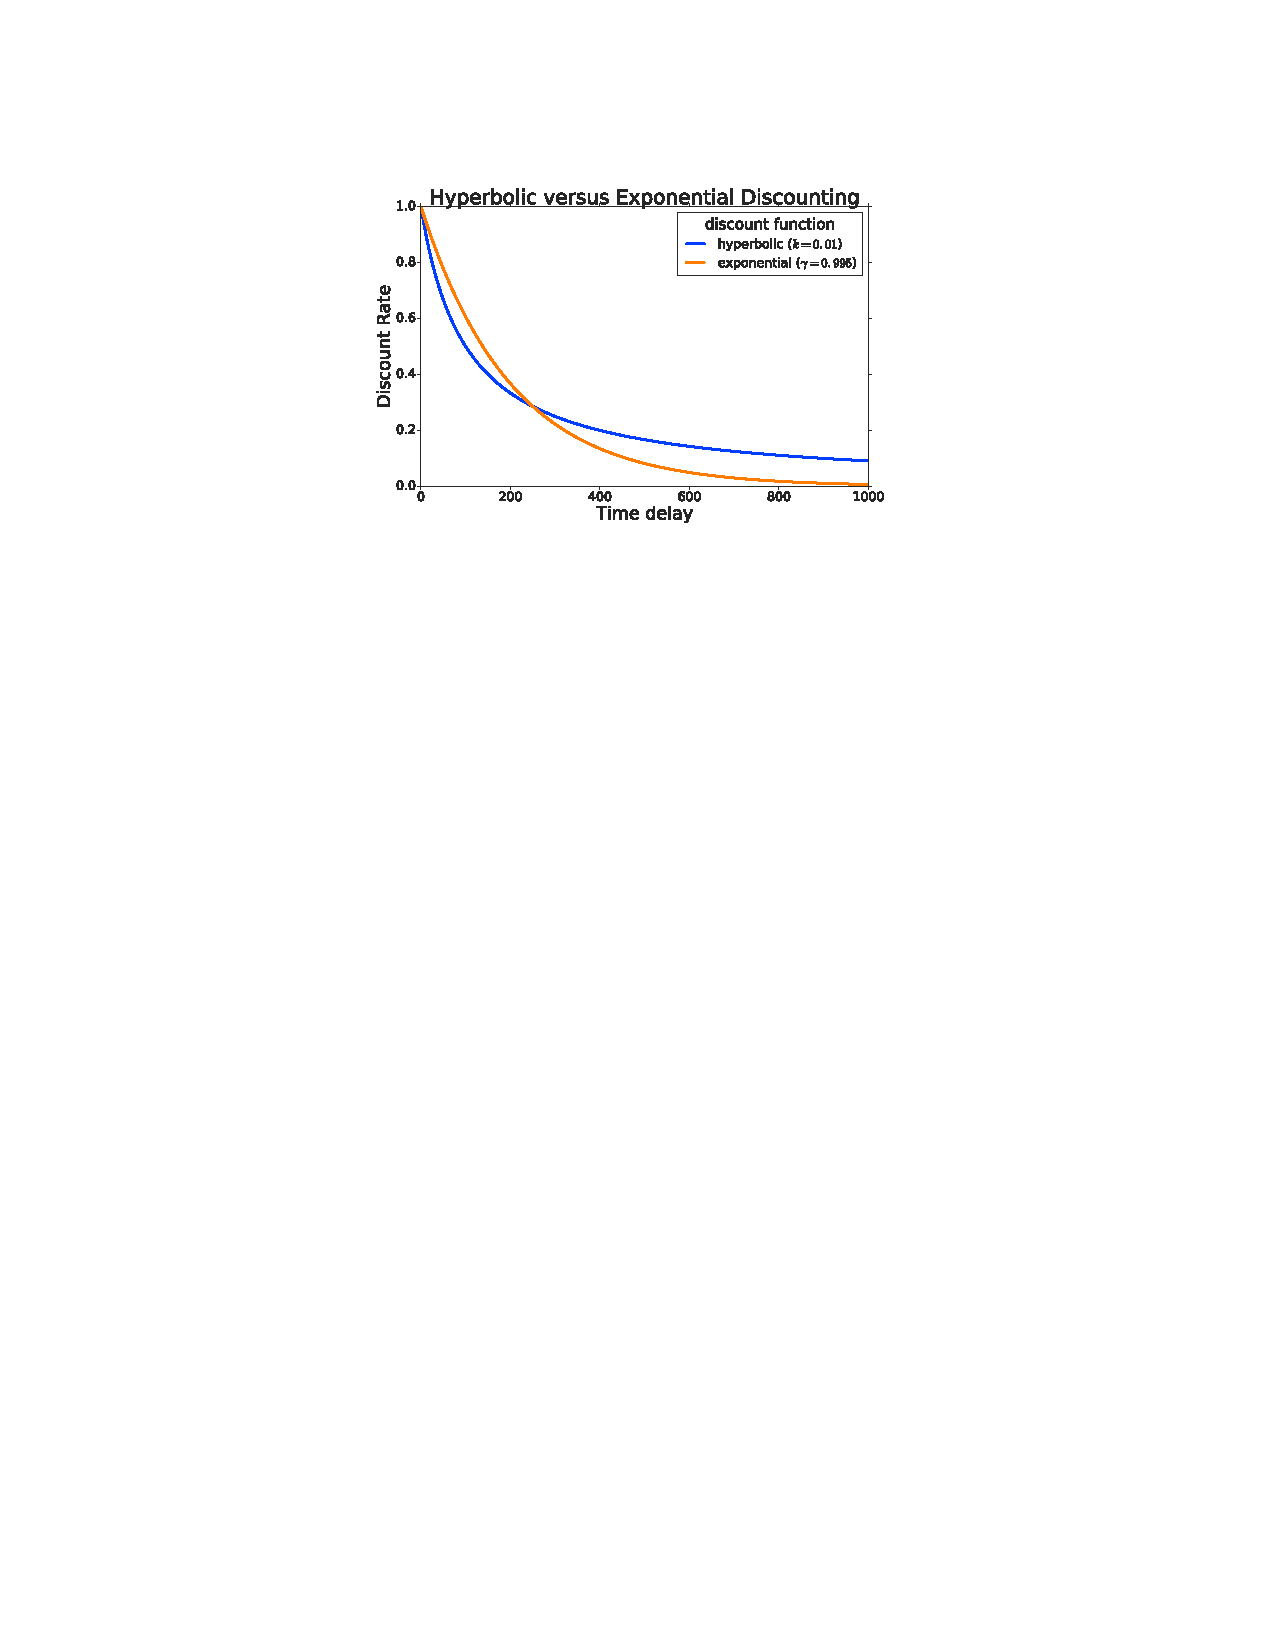
\includegraphics[width=0.5\textwidth]{images/disc.pdf}
    \caption{Hyperbolic vs. Geometric discounting, image from~\citet{fedus2019hyperbolic}}
    \label{fig:my_label}
\end{figure}

Suggestion: Future rewards are discounted based on probability of surviving to collect them: 
\[
v(r_t) = s(t) r_t,
\]
with $s(t)$ some survival probability. From:
\ddef{Survival Rate}{Survival $s(t)$ is the probability of agent surviving until time $t$:
\[
s(t) = \Pr(\tx{agent is alive at time t})).
\]}
Basically, hazard rate prior implies a discount function~\cite{sozou1998hyperbolic}. \\

$\ra$ Let's use these insights to understand RL in hazardous environments:
\[
s(t) = (e^{-\lamnda})^t = (\gamma)^t.
\]
Agent subject to a per time step probability of dying, or continuing probability of gamma. \\

\ddef{Hazardous MDP}{A hazardous MDP is an episodic POMDP: a hazard rate is sampled from a hazard distribution
\[
\lambda \sim H,
\]
with a modified model:
\[
P_\lambda(s' \mid s,a) = e^{-\lambda}P(s' \mid s,a).
\]}

Yield hazards Q:
\[
Q_\pi^{H,d}(s,a) = \bE_\lambda \bE_\pi\left[ \ldots \right].
\]

{\bf Contribution 1:}
\begin{lemma}
If there exists a function $w : [0,1] \ra \mathbb{R}$ such that:
\[
d(t) = \int_{\gamma=0}^1 w(\gamma) \gamma^t d\gamma, 
\]
then there is a well formed Q function:
\[
Q_\pi^{H,d}(s,a) = \int_{\gamma=0}^1 w(\gamma) \gamma^t Q_\pi^{H,\gamma}(s,a) d\gamma, 
\]
\end{lemma}

Practically speaking: for a given state, we model value over multiple time horizons. \\

{\bf Contribution 2:} Multi-horizon auxiliary task. \\
\begin{itemize}
    \item Experiments in Atari.
    \item One finding: compare hyperbolic use of discount vs. using a large $\gamma$---in both cases, find improvements in some subset of tasks.
    \item Ablation Study: use C51 by~\citet{bellemare2017distributional}, with multi-horizon auxiliary task.
    
    $\ra$ Auxiliary task does not interface well with a prioritized replay buffer. 
    
\end{itemize}

{\bf Conclusions:} Growing tension in time-preferences in RL! See work by: \citet{pitis2019rethinking,white2017unifying}.

Contributions:
\begin{enumerate}
    \item Practical and efficient approach for training deep RL agents with hyperbolic and other non-exponential time-preferences.
    
    \item Modeling the world over multiple time-horizon improves learning dynamics (serves as a useful auxiliary task).
\end{enumerate}
 
 \spacerule
 
 \subsection{Susan Murphy on RL for Mobile Health}

Goals of mobile health:
\begin{enumerate}
    \item Promote behavior change and maintenance of this change (assist user in achieving long term goals, manage chronic illness, and so on).
    \item Test, evaluate, develop causal science.
\end{enumerate}

Two kinds of actions in mobile health: 1) Pushes and 2) Pulls. \\

$\ra$ Pull: when you go to the resource for finding information/help.  Requires that the individual recognize they need help and take action. \\

$\ra$ Push: the app itself takes action to help or intervene. Can be aggravating, though.

{\bf Focus here:} pushes! Because, more opportunity for impact in the long run. \\

Experimental flavor: micro-randomized trial:
\begin{itemize}
    \item Each user is randomized many time: sequential experimentation
    \item Sequential experimentation may use online predictions as well as RL
\end{itemize}


{\bf Study 1:}
\begin{itemize}
    \item Individuals that want to quit smoking wear a bunch of smoking.
    \item Goal is to provide signals infrequently that can help individuals when stressed. Suppose you only get one intervention a day.
    %\item Sense$^2$Stop MRT for stress management in newly abstinent smokers
    \item Setup: treat this is an RL problem!
    \item Data: time series $(s,a,r,s')$ of trajectories taken, with actions a treatment push, $s$ the context of user data.
\end{itemize}


Two (of many!) Mobile Challenges in RL:
\begin{enumerate}
    \item Highly variable context/rewards and potentially complex reward function
    \item Treatments that tend to have positive effects on immediate rewards (relative to no treatment) but negative impact on future rewards via user habituation/burden.
    
    $\ra$ Lots of delayed effects!
\end{enumerate}

{\bf Mobile App: HeartSteps:}
\begin{itemize}
    \item Goal: develop a mobile activity coach for individuals who are at high risk of adverse cardiac events
    \item Results from V1: micro-randomized studies to determine how people get randomized.
    \begin{itemize}
        \item Lots of different treatments available, operate at different time scales.
        \item Focused on an individuals schedule, context, and so on.
        \item Actions are to deliver (or not) a tailored message to encourage user to be more active 9for example).
        
        $\ra$ Example message: Hey, look outside! Not so bad? Maybe you can walk to work today?

        \item Finding 1: tailored activity suggestion (compared to no activity) more than {\it doubled} their step count over next 30 minutes. Increase dissipated over time, though $\ra$ likely due to habituation. 
        \item Finding 2: Number of features that predict 30 minute step count include time in study, recency-discounted message dose, location, total steps on prior day, temperature.
        
        $\ra$ Time in study is particularly problematic, as it highlights non-stationarity in the reward function!
    \end{itemize}
    
    \item {\bf Goal of V2:} Use an RL algorithm to decide whether or not to intervene.
    
    \begin{itemize}
        \item Study carried out over three months this time (much longer than V1).
        \item Went with a more bandit-like algorithm: model mean reward given the treatment and features $(s,a)$.
        \item Use a linear model for mean reward, use linear Thompson sampling-like approach (track posterior distribution over payoffs, use posterior sampling to act).
    \end{itemize}

\end{itemize}

Return to the two challenges: 1) high variance in rewards/contexts, 2) lots of delay. \\

$\ra$ One solution: Bandits! In a bandit, can learn faster because the bandit acts as a regularizer ($\gamma = 0$). \\

$\ra$ Another solution: Informative prior on unknown parameters. Gaussian prior where parameters determined by the V1 trial. \\

Delayed effects are challenging, too: requires rethinking posterior sampling a bit. \\

$\ra$ Solution: modify Thompson sampling treatment selection probabilities. Built a low-dimensional proxy MDP in which dose $d$ evolves deterministically and all other states are i.i.d. across time. \\

New learning algorithm: Bayesian linear regression (aka Gaussian Processes). \\

$\ra$ Evaluation: 3-fold cross validation performance relative to Thompson sampling with V1. \\

{\bf Open Questions:}
\begin{itemize}
    \item What should the optimality criterion be in a study like these? (That is, we know there will be clinical trials at the end). How can we design the study itself to minimize regret?
    
    $\ra$ Idea: Maximize finite time $T$ total reward subject to bounds on power to detect a particular causal effect at time $T$.
    
    $\ra$ Often multiple goals for a learning algorithm.
    
    \item Often need intermittent off-policy inferences: 1) permit causal inference, 2) concern different outcomes than the reward, 3) use different model assumptions, and so on.
    
    \item Generalization of RL to include very different treatment classes, occurring at different time scales and targeting different outcomes/rewards.
\end{itemize}


\spacerule

\subsection{Liyu Xia on Option Transfer in Humans}

Joint work with Anne Collins. \\

{\bf Theme:} Hierarchical human behavior. People are very good at breaking down complicated tasks into simpler ones. \\

$\ra$ This work: can we understand this process quantitatively? \\

Options framework: augment the agent's action space $\mc{A}$ with a set of high level actions called {\it options} \cite{sutton1999between}.

\ddef{Option}{An option is a triple: $o = \langle \mc{I}, \beta, \pi \rangle$ denoting the initiation condition, termination condition, and policy, respectively.}

Q: How do options fit into human behavior? \\

A: Consider the task of making coffee/making toast. Both of these can be decomposed into simpler subproblems like cutting bread, boiling water, and so on. \\

$\ra$ Can transfer at multiple levels of abstraction. Options can give us a theoretical framework for supporting this kind of transfer of subtrask structure. \\

Questions studied in this work;
\begin{itemize}
    \item Do we as humans use options through RL? How about options of options?
    \item Can we transfer options? At any level?
    \item Does option improve exploration and speed up human learning?
\end{itemize}

To address these questions $\ra$ a new experimental design. Idea:
\begin{itemize}
    \item Two stages: 10 Given a stimuli (picture of circle), must press some key in response to advnace (up arrow), then 2) Next stage, see a different shape which requires a different button to be pressed.
    \item Second stage is random to rule out pure sequence learning, and second stange depends on first stage.
    
    \item 60 trials of the above two stages constitutes a single ``block".
    
    \item Crucial aspect of the design: action assignments. Unsignaled context, creation of two sets of high level options, then reactive high-level options in later blocks.
    
    \item The test: can subjects positively transfer low-level options? Is there negative transfer as a result of transferring high-level options?
\end{itemize}


General Behavior: count the average number of key presses per ``block" to measure ho well participants can learn the task. \\

$\ra$ In later blocks (5-8, later stages of learning): evidence that participants are in fact learning and transferring options (both positively and negatively, in some cases). \\

Modeling: use a {\it chinese restaurant process} (CRP)---roughly, what is the probability that a new customer at a restaurant ends up sitting at a particular table? \\


Experiments: option model tends to predict human transfer effects quite well. \\

Summary:
\begin{itemize}
\item Behavioural signatures of option learning and transfer through a new behavioral paradigm
\item The option model + CRP is human-like and enables flexible option trasnfer at multiple levels
\item Three more experiments testing other aspects of options, naturalistic, compositional, and so on.
\end{itemize}

\spacerule

\subsection{Yash Chandak on Improving Generalization over Large Action Sets}

Joint work with Georgious Theocharous, James Kostas, Scott Jordan, and Philip Thomas. \\

Q: When an action is executed, what can we say about any actions {\it not taken}? \\

A: Could be really important! Think about a tutoring system---millions of possible actions (lessons) to choose from. Should be really important to learn about how actions relate to one another. Also relevant in: advertising, medical treatment, portfolio management, song recommendation, and so on. \\

\dbox{{\bf Central Question:} When we have a huge number of actions, how do we learn efficiently?}

Key insight from prior work: state representations help in generalizing feedback across larse state sets. \\

But! What can we learn about generalizing feedback across large action sets. \\

**Actions are not independent discrete quantities. They likely have some low dimensional structure underlying their behavior pattern. \\

Note: With both state and action representations we often want a representation that is reward-function agnostic. \\

New paradigm: break the agent into three pieces: 1) $\pi_i$, which yields an action, 2) $e$, which maps actions into some latent action representation space, and 3) $f$ which maps an action in this space into the actual action space. \\

Policy decomposition:
\[
\pi_o(a \mid s) = \int_{f^{-1}(a)} \pi_i(e \mid s) de.
\]
Q: Why do we need the policy itself?\\

A: Well, two reasons: 1) to execute, and 2) to learn. But, the above integral presents a big computational bottleneck. Turns out we can actually avoid this entirely. \\

Q: So how do we learn these action representations? \\

A: Supervised learning! Want a pair of functions $g,f$ that map actions into a latent space ($e_t$), and then move these ``latent" actions back to the original space. Our data is the usual $s_t, a, s_{t+1}$. We now want to predict which action (in this latent space) is responsible for the given transition. \\

$\ra$ Can then learn an internal policy with policy gradients. \\

Q: So, did it work? \\

A: Toy maze with continious state and $n$ actuators that propell the agent into a particular direction. Compare an Actor-Critic to an Actor-Critic with representations for actions (ACRA). \\

Results: with a small domain, both approaches perform well. With a larger domain, though, the baseline completely fails whereas the ACRA tends to do quite well even with a high dimensional action space. \\

{\bf Adobe Experiments;} Multi-time step user behavior model. Achieve similar results to the maze; ACRA performs well despite the large action space. \\

Summary: 1) We should exploit structure in action space, 2) generlization of feedback to similar actions, 3) less parameters updated using high variance policy gradients, 4) complementary to state representations. \\

\spacerule

\subsection{Shiela Mcilrath on Reward Machines}

Joint work with Rodrigo Toro Icarte, Toryn Klassen, Richard Valenzano, Alberto Camacho, Leon Illanes, Xi Yan, Ethan Waldie, and Margarita Castro. \\

{\bf Language is Critical:} Humans have evolved language over thousands of years to provide useful abstractions for understanding and interacting with each other and with the physical world. Roughly 6500 spoken langages in the world. Claim advanced by some is that language influences what we think, what we perceiv, how we focusour attention, and what we remember. \\

\dbox{{\bf Central Question:} Can exploiting the alphabet and structure of language help RL agents learn and think?}

$\ra$ How do we advice, instruct, task, and impart knowledge to our RL agents? \\

Consider typical goals and preferences:
\begin{itemize}
\item Run the diswhaser when it's full or when dishes are needed for the next meal.
\item Make sure the bath temperature is between 38-43 celcius before letting someone enter.
\item Do not vacuum when someone is sleeping.
\item When getting ice cream, please open the freezer take out the ice cream, serve yourself, put the ice cream back in the freezer, and close the freezer door.
\end{itemize}

One idea for specifying tasks: linear temporal logic! Some additional semantics/syntax added to first order logic that allows for explicit description of temporal properties like ``eventually", ``always', and so on. \\

$\ra$ Example 1: do not vacuum while someone is sleeping:
\[
\tx{always}[ \neg (\tx{sleeping} \wedge \tx{vacuum})].
\]

Challenges in RL:
\begin{enumerate}
\item {\bf Reward Specification:} hard to pin down the right reward function for complex tasks.
\item {\bf Sample Efficiency}
\end{enumerate}

Running Example: a patrol task in a grid world. Agent has to move around a series of rooms in sequence, then gets a reward (and then should repeat this process) \\

$\ra$ Dirty secret: environment doesn't give reward! We do. We have to write a reward function somewhere. \\

{\bf Simple Idea:} Give agent access to the rward function and exploit reward function structure in learning. \\

$\ra$ Main mechanism for doing this is a reward machine. \\

\ddef{Reward Machine (RM)}{An automata like structure that characterizes a reward function. Consists of: finite set of states $\mc{U}$, initial state $u_0 \in \mc{U}$, and a set of transitions labelled by a logical condition and reward functions.}

Really, then, a reward machine is a ``Mealy" machine over the input alphabet whose output alphabet is a set of Markovian reward functions.\\

Example: Back to the patrol case. Three rooms in the grid world, A, B, and C. The reward machine is a simple automata that provides reward depending on which room the agent is in (and the relevant state variables denoting where the agent has been). Agent receives reward every time the sequence $A \ra B \ra C$ is visited.

\subsubsection{Using Reward Machines in Learning}

Q: How can we exploit Reward Machine structure in learning? \\

A: Five variaitions.
\begin{enumerate}
\item (Q-Learning) Q-Learning over an equivalent MDP
\item (HRL) Hierarchical RL based on options
\item (HRL+Rm) Hierarchical RL with reward machine based pruning
\item (QRM) Q-Learning for reward machines.
$\ra$ Give this structure to the learning algorithm to exploit during learning. Learn one policy per state in the reward machine, then select actions using the policy of the current RM state (also reuse experience and do off-policy updates).
\item (QRM+RS) Q-Learning for reward machines with reward shaping.
$\ra$ Do VI over the MDP induced by the RM to compute a nice shaped reward function, inject that reward into the RM.
\end{enumerate}

Note that HRL methods can find suboptimal policies by only optimizing locally. \\

{\bf Experiments:} two domains with discrete state-action spaces, some minecraft like problem, and a continuous state space.

\begin{enumerate}
\item Office domain (patrol task): QRM learns extremely quickly, HRL+RM also learns quite quickly.
\item Minecraft-esque domain (10 tasks, 10 random maps); Q-Learning can't learn at all given the budget, QRM is extremely efficient again along with HRL+RM.
\item Extension of QRM to Deep QRM: Replace Q-Learning with Double DQN with priorized experience replay.

$\ra$ Water world: color balls bouncing off of some walls in a 2d continuous environment. Agent (which is itself a ball) has to hit two red balls, hit a green ball, and so on.

$\ra$ Again find QRM (in this case DQRM) works quite well. Hierarchical method works relatively well, too.

\item Final experiment: explore the effect of the shaping on performance. Reward shaping almost always helps (faster learning), but in continuous state domain (water world) shaping doesn't help.
\end{enumerate}


\subsubsection{Creating Reward Machines}
Q: where do RMs come from?
\begin{enumerate}
\item A1: Specified by hand!

$\ra$ Can specify reward-worthy behavior in any formal language translatable to finite state automata. Many of these languages are natively declarative and composable.

\item A2: Generate RM from high level goal specification (symbolic planner).

$\ra$ Employ explicit high-level model to describe abstract actions, use abstract solutions to guide an RL agent.

\item A3: Learn them from data.

$\ra$ Find a policy that maximizes the collected external reward given by a partially observable environment.

$\ra$ Key insight: learn an RM such that its internal state can be effectively used as external memory by the agent to solve the task.

\end{enumerate}

Summary:
\begin{itemize}
    \item Main Q: can exploiting the alphabet and structure of language help RL agents learn and think?
    \item Key insight: reveal reward function to the agent (via reward machines)
    \item Using RMs can serve as a normal form representation for reward functions.
\end{itemize}

\spacerule


\subsection{Poster Spotlights}

Next up we have quick poster spotlights (two minute talks):
\begin{enumerate}
\item Kearney et al.: Making meaning: Semiotics within predictive
knowledge architectures.

$\ra$ Study of signs and symbols (semiotics) could inform the analysis and design of predictive knowledge architectures.

\item Holland et al.: The effect of planning shape on Dyna-style
planning in high-dimensional state spaces.

$\ra$ Given limited resources, how do we use the model to perform updates that are most effective?

\item Song et al.: Not smart enough: most rats fail to learn a
parsimonious task representation.

$\ra$ Can animals (rats) learn shared reward structure and use it for faster learning and better decisions? Short answer: No, they can't!

\item P{\" a}rnamets et al.: Learning strategies during repeated
spontaneous and instructed social avoidance learning.

$\ra$ two questions: 1) how do people learn from social partners, and 2) how is this learned information used?

\item Islam et al.: Doubly robust estimators in off-policy actor critic algorithms.

$\ra$ Despite being sample efficient, off-policy learning can suffer from high variance. This work: extend doubly robust estimation to off-policy actor-critic to achieve low variance estimates in critic evaluation.

\end{enumerate}


And that's a wrap for Monday!


\spacerule



